\documentclass{article}

\usepackage{amsmath,amssymb}
\usepackage{graphicx}

\renewcommand{\P}{\mathbb{P}}
\newcommand{\D}{\mathbb{D}}
\newcommand{\Bin}{\operatorname{Bin}}

\newtheorem{remark}{Remark}

\title{Bergman $\beta$ Heuristic}
\author{}
\date{}

\begin{document}

\maketitle

The goal of this short note is to provide a heuristic explanation for why the limit(s) of finite-particle log gases in the disk are empty for $\beta>4$.

Recall that we consider the Gibbs point process
\[
\P_n(d\gamma)
=
\frac{1}{Z_{N,\beta}}
e^{-\beta H(\gamma)}
\Bin_{\D,n}(d\gamma),
\]
where $\Bin_{\D,n}$ is the $n$-point binomial point process in the unit disk $\D$, and
\[
H(\gamma)
=
-\sum_{\{x,y\}\subset\gamma}\log |x-y|.
\]

For a class $\mathcal{C}$ of configurations such that, for all
$\gamma\in\mathcal{C}$,
\[
H(\gamma)\simeq \mathrm{Cst},
\]
the restricted free energy is given by
\[
F_{n,\beta}(\mathcal{C})
:=
-\frac{1}{\beta}
\log\!\int_{\mathcal{C}}
e^{-\beta H(\gamma)}
\,\Bin_{\D,n}(d\gamma)
\simeq
\mathrm{Cst}
-\frac{1}{\beta}
\log \Bin_{\D,n}(\mathcal{C}).
\]

This quantity allows us to compare the probabilities of different classes of configurations. We know, at least for $\beta=2$, that almost all particles concentrate near the boundary of the disk. Because of the repulsion, it is reasonable to expect the points near the boundary to be distributed approximately evenly.

To understand where the transition at $\beta=4$ comes from, we compare the asymptotics of two candidate typical configurations:
\begin{enumerate}
    \item Configurations in which all particles approach the boundary, leaving an empty interior in the limit.
    \item Configurations in which essentially all particles lie near the boundary, while one particle remains near $0$.
\end{enumerate}
We will see that, for $\beta>4$, the free-energy cost of candidate~1 is favorable. This suggests an empty limiting point process.

Let us define the two corresponding classes of configurations, $\mathcal{C}_1$ and $\mathcal{C}_2$.

Let $n\geq 2$, and denote by
\[
\Gamma_n
:=
\{\gamma\subset\D:\#\gamma=n\}
\]
the space of configurations with $n$ points in the unit disk.

For $m\geq 1$, write
\[
\zeta_k^{(m)}
:=
e^{2\pi i k/m},
\qquad
k=0,\ldots,m-1.
\]

We define the reference class $\mathcal{C}_1$ by
\[
\mathcal{C}_1
:=
\left\{
\gamma\in\Gamma_n:
\#\bigl(\gamma\cap B(\zeta_k^{(n)},1/n)\cap\D\bigr)=1
\text{ for } k=0,\ldots,n-1
\right\}.
\]

\begin{remark}
Of course, a typical boundary configuration would instead be some random rotation of a configuration resembling $\mathcal{C}_1$. The computation can be carried out for a more general class of configurations, but doing so does not provide additional insight. Moreover, we compare $\mathcal{C}_1$ with a class having the same type of ``fixed reference.'' Thus, the entropy lost by not taking this random permutation into account is, to some extent, compensated by making the same restriction for $\mathcal{C}_2$.
\end{remark}

The figures illustrate the case $n=10$. Black dots represent particles, while hollow circles mark the centers of the balls.

\begin{center}
    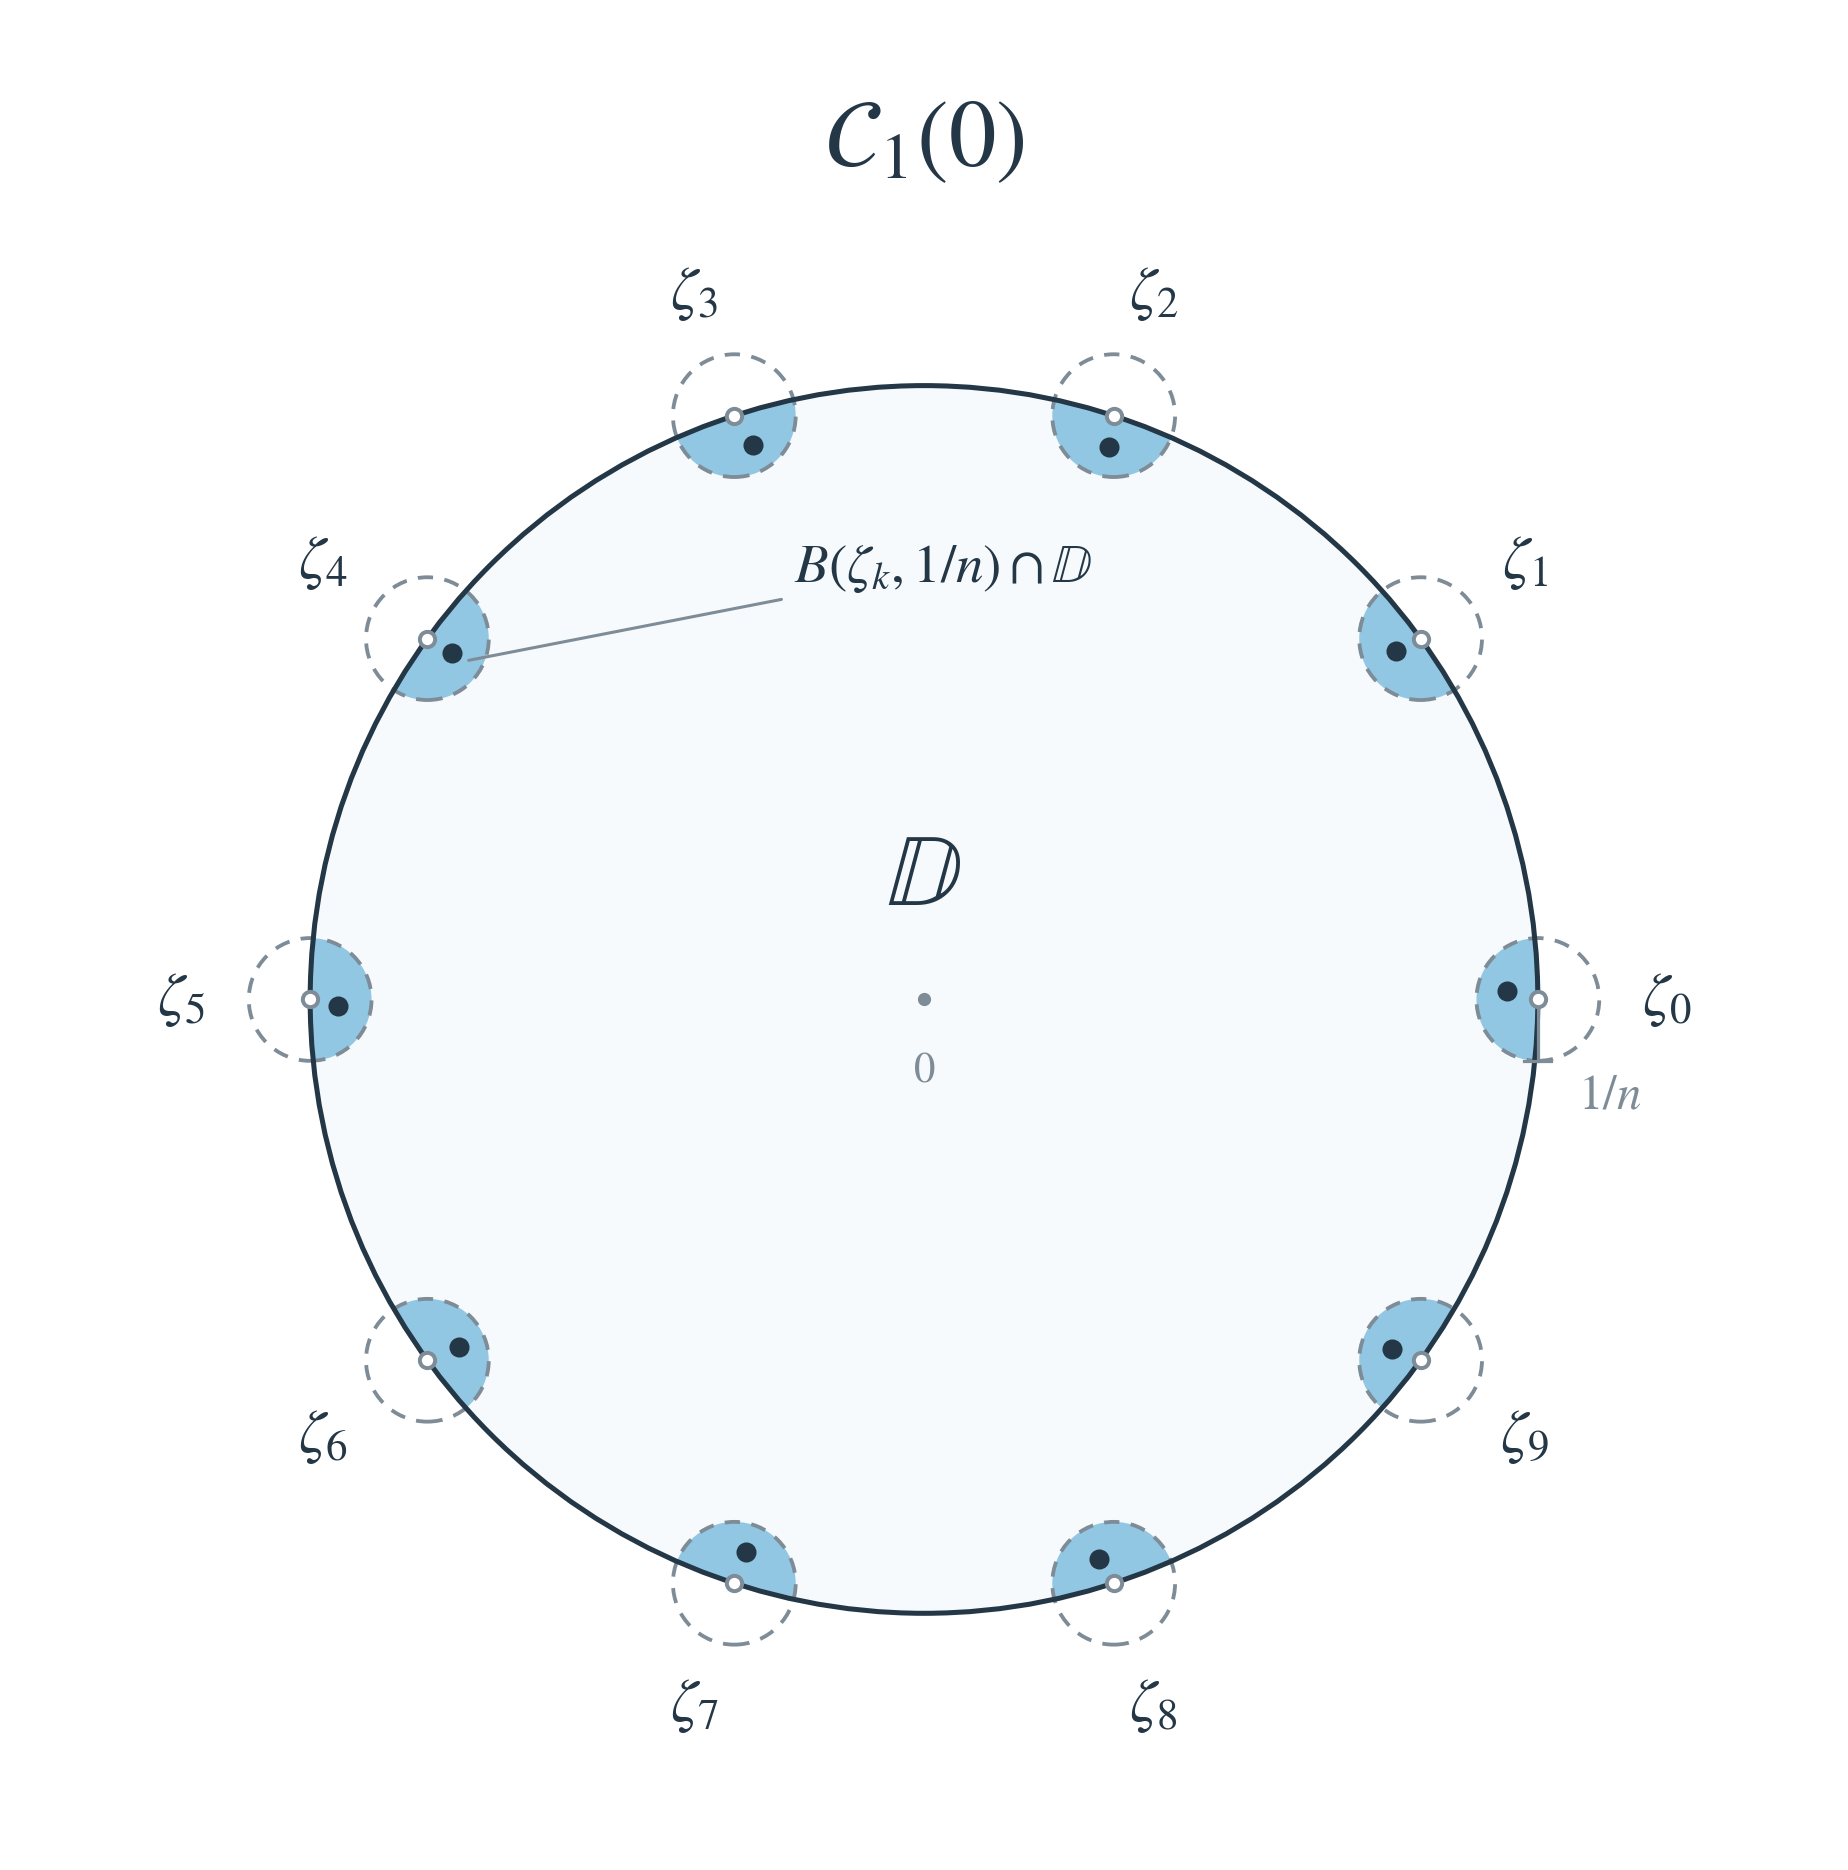
\includegraphics[width=0.65\textwidth]{Assets/class1.png}
\end{center}

Thus, there is exactly one point in each blue boundary region and no points elsewhere.

\begin{center}
    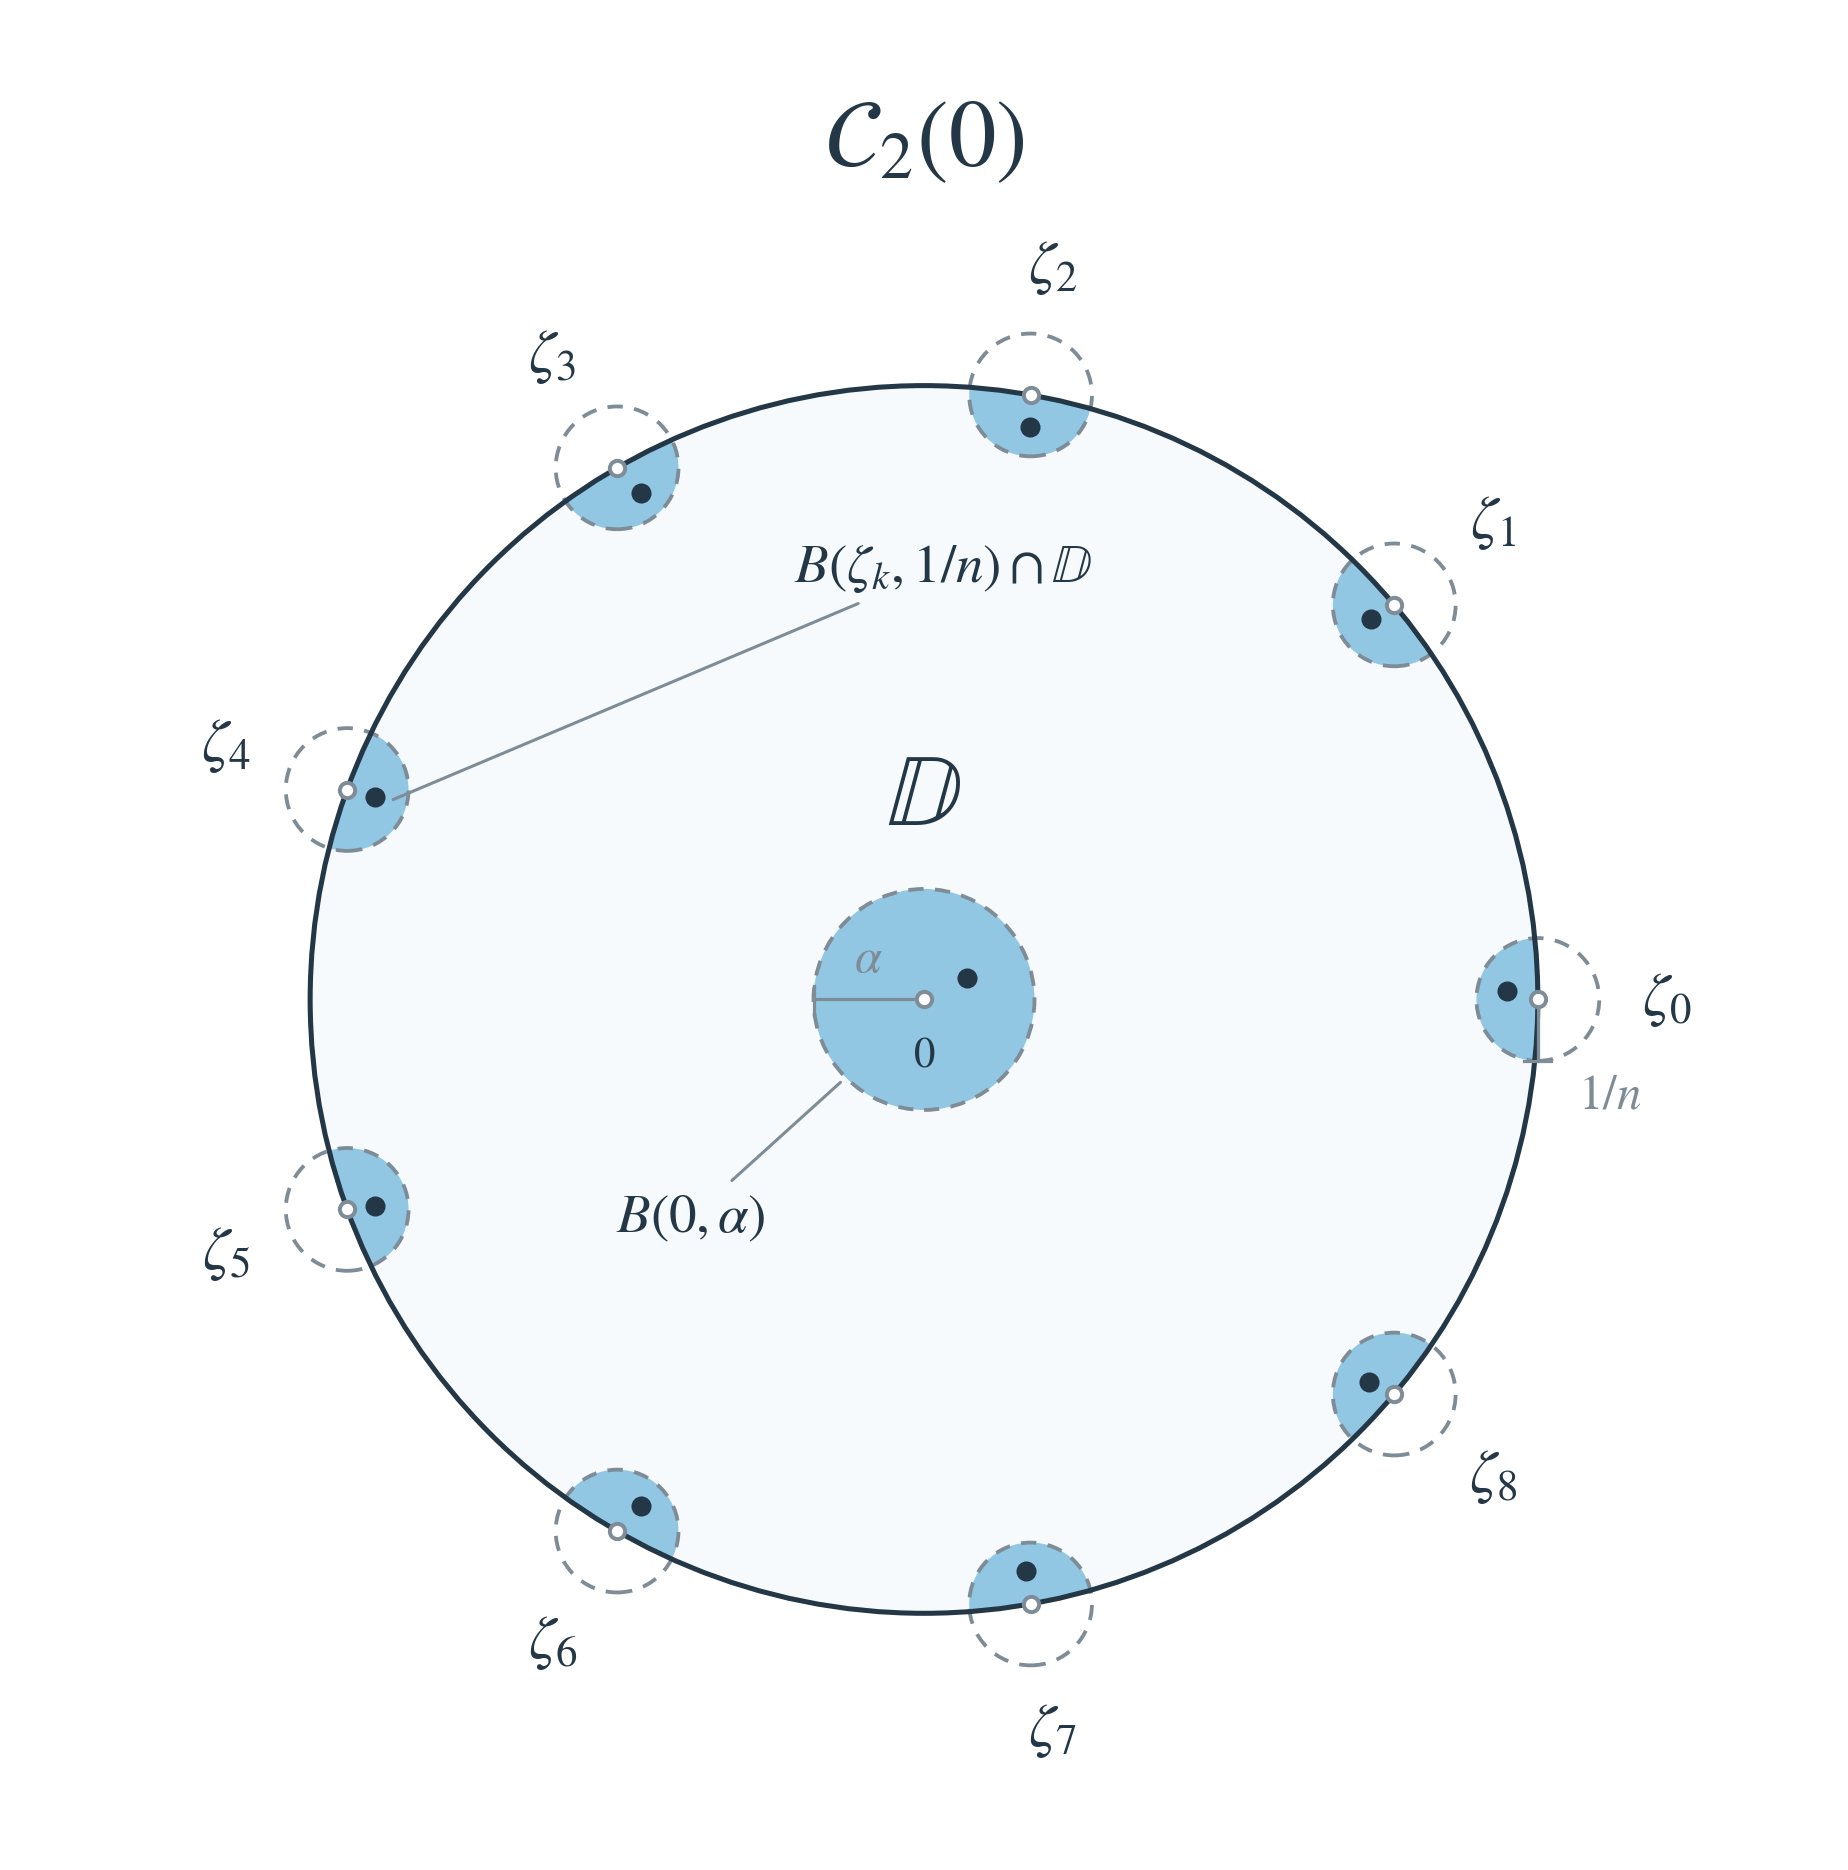
\includegraphics[width=0.65\textwidth]{Assets/class2.png}
\end{center}

Let $\alpha>0$ be small. Similarly, we define the reference class $\mathcal{C}_2$ by
\[
\mathcal{C}_2
:=
\left\{
\gamma\in\Gamma_n:
\begin{array}{l}
\#\bigl(\gamma\cap B(0,\sqrt{\alpha})\bigr)=1,\\[2pt]
\#\bigl(\gamma\cap B(\zeta_k^{(n-1)},1/n)\bigr)=1
\text{ for } k=0,\ldots,n-2
\end{array}
\right\}.
\]

Thus, there is exactly one point in the central ball and one point in each of the $n-1$ blue boundary regions, with no points elsewhere.

We now compute the binomial probabilities of these two classes. Write $|E|$ for planar area and set
\[
q_n
:=
\frac{|B(1,1/n)\cap\mathbb{D}|}{\pi}.
\]

Thus, $q_n$ is the contribution of one boundary cap, while the central ball contributes $\alpha/\pi$.

We then have
\[
\Bin_{\mathbb{D},n}\bigl(\mathcal{C}_1\bigr)
=
n!\,q_n^n,
\qquad
\Bin_{\mathbb{D},n}\bigl(\mathcal{C}_2\bigr)
=
n!\,\alpha q_n^{n-1}.
\]

We have
\[
q_n
\simeq
\frac{1}{2n^2}.
\]

Hence,
\[
\Bin_{\mathbb{D},n}(\mathcal{C}_1)
\simeq
n!\,2^{-n}n^{-2n},
\qquad
\Bin_{\mathbb{D},n}(\mathcal{C}_2)
\simeq
n!\alpha \,2^{1-n}n^{2-2n}.
\]

Set
\[
\gamma_1^{(n)}
:=
\{\zeta_0^{(n)},\ldots,\zeta_{n-1}^{(n)}\},
\qquad
\gamma_2^{(n)}
:=
\{0,\zeta_0^{(n-1)},\ldots,\zeta_{n-2}^{(n-1)}\}.
\]
These are the prototypical configurations associated with $\mathcal{C}_1$ and $\mathcal{C}_2$, respectively.

Because of the repulsion, we expect the points near the boundary to be distributed close to $\gamma_1^{(n)}$ and $\gamma_2^{(n)}$. We therefore use the approximations
\[
H(\gamma)
\simeq
H(\gamma_i^{(n)}),
\qquad
\forall\,\gamma\in\mathcal{C}_i,
\qquad
i\in\{1,2\}.
\]

The classical computation gives
\[
H(\gamma_1^{(n)})
=
-\frac{n}{2}\log n
\]
and
\[
H(\gamma_2^{(n)})
=
-\frac{n-1}{2}\log(n-1).
\]
The contribution of the central point disappears because the $\zeta_k$'s are roots of unity.

In particular,
\[
H(\gamma_1^{(n)})-H(\gamma_2^{(n)})
=
-\frac{1}{2}\log n-\frac{1}{2}+O(n^{-1}),
\qquad
n\to\infty.
\]

Thus, the free-energy discrepancy is
\[
\Delta_n
:=
F_{n,\beta}(\mathcal{C}_1)
-
F_{n,\beta}(\mathcal{C}_2)
=
\left(\frac{2}{\beta}-\frac{1}{2}\right)\log n
+O(1).
\]

Hence, for $\beta<4$, $\Delta_n\to+\infty$, whereas for $\beta>4$, $\Delta_n\to-\infty$. Thus, in the first case, $\mathcal{C}_2$ is more favorable, while in the second case, $\mathcal{C}_1$ is favored.

\end{document}